% Requires graphicx and booktabs. Paths are relative to analysis_sol_output.
\section{Results}
\subsection{Data completeness and exclusions}
Of 225 intended observations from 45 benchmark cases, 220 evaluations had all three scores and 5 failed. The primary analysis retained 44 complete cases (220 observations). Excluded cases: Cruise. Recorded reasons: ValueError: Unrecognized line 51: '<> diamond'. A parser error does not by itself identify whether the reference or generated diagram caused the failure.
\subsection{Baseline scores and repeated-generation variability}
Associations: mean 0.755 (SD 0.141; range 0.424--0.994); Attributes: mean 0.787 (SD 0.146; range 0.401--0.994); Classes: mean 0.777 (SD 0.139; range 0.418--0.982)
. 
\begin{center}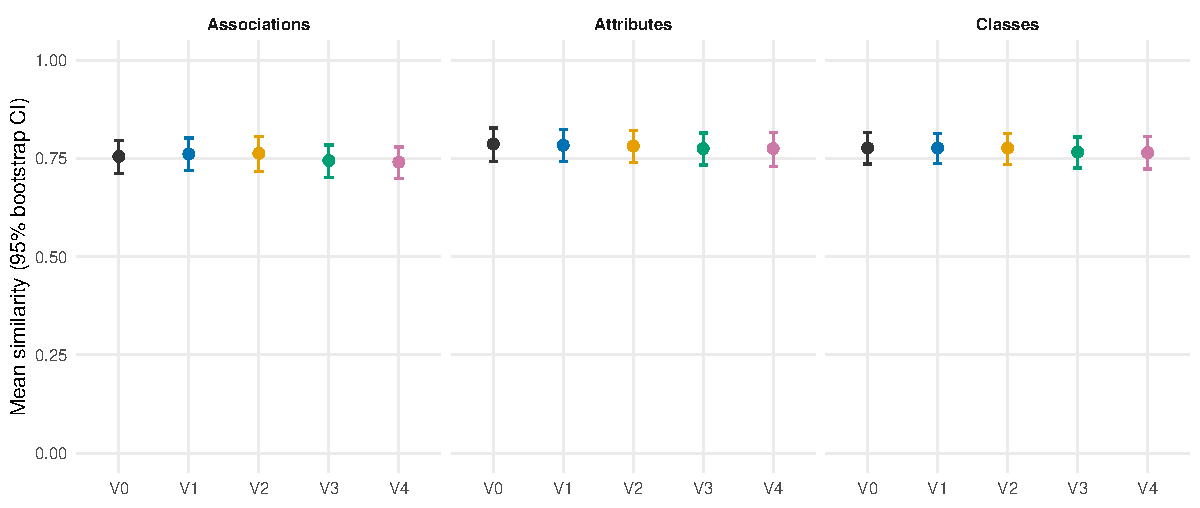
\includegraphics[width=\linewidth,height=0.30\textheight,keepaspectratio]{figures/fig1_condition_means.pdf}\par\small Condition means with pointwise 95\% case-bootstrap intervals; complete cases only.\end{center}
Associations: signed mean -0.001, mean absolute difference 0.035 and median absolute difference 0.029 (6/44 exactly identical); Attributes: signed mean -0.004, mean absolute difference 0.032 and median absolute difference 0.019 (11/44 exactly identical); Classes: signed mean -0.003, mean absolute difference 0.030 and median absolute difference 0.020 (5/44 exactly identical)
. Replication statistics use all available paired baseline scores. They quantify empirical repeated-generation variability, not a formal detection threshold.
\newpage
\subsection{Effects of textual conditions}
V1 makes information implicit, V2 introduces ambiguity, V3 introduces a semantic anomaly, and V4 paraphrases the description. All differences are variant minus V0; negative values indicate lower reference similarity. Two-sided Wilcoxon signed-rank tests use tie and continuity corrections, with Holm adjustment over twelve tests. Signed-rank location inference assumes symmetric differences. Bootstrap intervals describe arithmetic mean differences and are pointwise, not multiplicity-adjusted.
\paragraph{Classes.} V1: mean difference -0.000, 95\% CI [-0.018, 0.016], median 0.000, Holm-adjusted $p$ 1.000; V2: mean difference -0.001, 95\% CI [-0.011, 0.009], median 0.000, Holm-adjusted $p$ 1.000; V3: mean difference -0.011, 95\% CI [-0.022, -0.001], median -0.001, Holm-adjusted $p$ 0.960; V4: mean difference -0.012, 95\% CI [-0.026, 0.001], median -0.014, Holm-adjusted $p$ 0.341.
\paragraph{Attributes.} V1: mean difference -0.003, 95\% CI [-0.023, 0.014], median 0.000, Holm-adjusted $p$ 1.000; V2: mean difference -0.005, 95\% CI [-0.015, 0.006], median 0.000, Holm-adjusted $p$ 1.000; V3: mean difference -0.011, 95\% CI [-0.022, -0.001], median -0.000, Holm-adjusted $p$ 0.929; V4: mean difference -0.011, 95\% CI [-0.026, 0.003], median -0.007, Holm-adjusted $p$ 0.563.
\paragraph{Associations.} V1: mean difference 0.006, 95\% CI [-0.014, 0.024], median 0.007, Holm-adjusted $p$ 1.000; V2: mean difference 0.008, 95\% CI [-0.006, 0.021], median 0.009, Holm-adjusted $p$ 0.911; V3: mean difference -0.010, 95\% CI [-0.027, 0.005], median 0.000, Holm-adjusted $p$ 1.000; V4: mean difference -0.015, 95\% CI [-0.032, 0.003], median -0.009, Holm-adjusted $p$ 0.960.
None of the twelve primary tests rejected after Holm correction. This does not establish zero effects or equivalence.
\begin{center}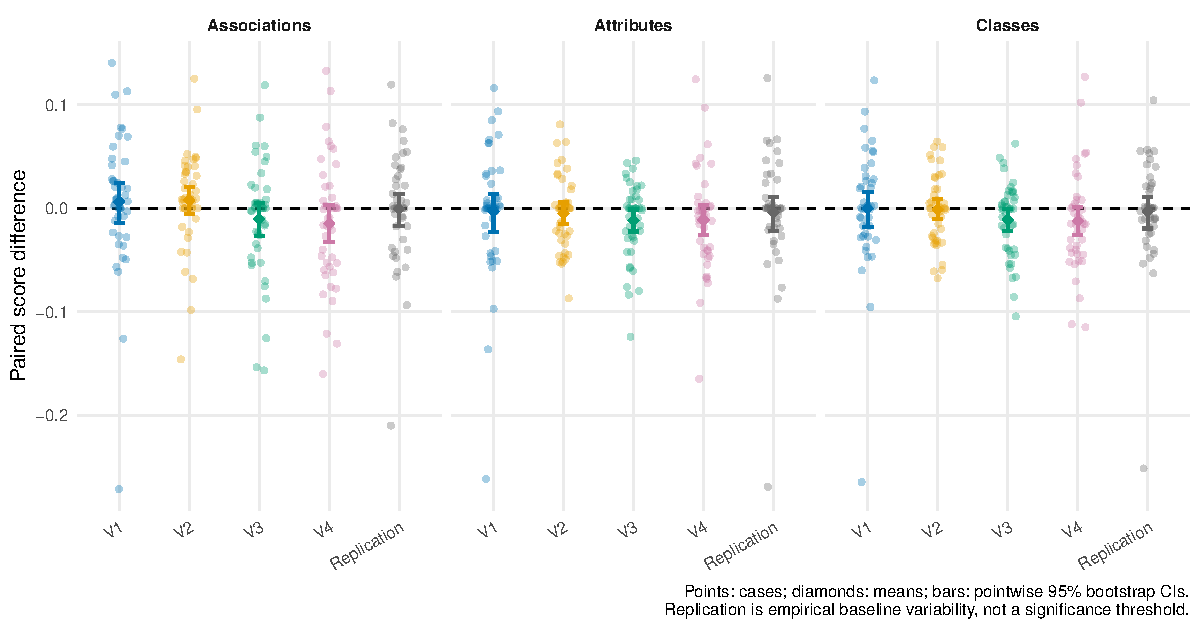
\includegraphics[width=\linewidth,height=0.30\textheight,keepaspectratio]{figures/fig3_effects_and_replication.pdf}\par\small Individual signed differences and mean estimates. The replication distribution is an empirical variability reference, not a statistical acceptance region.\end{center}
\newpage
\subsection{Condition effects relative to generation variability}
V1/Associations: mean absolute variant difference 0.042 versus replication 0.035 (paired excess 0.007, CI [-0.003, 0.017]); V1/Attributes: mean absolute variant difference 0.038 versus replication 0.032 (paired excess 0.006, CI [-0.005, 0.017]); V1/Classes: mean absolute variant difference 0.036 versus replication 0.030 (paired excess 0.007, CI [-0.001, 0.014]); V2/Associations: mean absolute variant difference 0.032 versus replication 0.035 (paired excess -0.003, CI [-0.017, 0.011]); V2/Attributes: mean absolute variant difference 0.027 versus replication 0.032 (paired excess -0.004, CI [-0.021, 0.009]); V2/Classes: mean absolute variant difference 0.025 versus replication 0.030 (paired excess -0.005, CI [-0.020, 0.007]); V3/Associations: mean absolute variant difference 0.038 versus replication 0.035 (paired excess 0.003, CI [-0.011, 0.017]); V3/Attributes: mean absolute variant difference 0.027 versus replication 0.032 (paired excess -0.005, CI [-0.021, 0.009]); V3/Classes: mean absolute variant difference 0.027 versus replication 0.030 (paired excess -0.003, CI [-0.017, 0.009]); V4/Associations: mean absolute variant difference 0.046 versus replication 0.035 (paired excess 0.011, CI [-0.004, 0.026]); V4/Attributes: mean absolute variant difference 0.035 versus replication 0.032 (paired excess 0.003, CI [-0.015, 0.019]); V4/Classes: mean absolute variant difference 0.036 versus replication 0.030 (paired excess 0.006, CI [-0.009, 0.020])
. Comparisons of absolute differences use the same cases on both sides and paired bootstrap intervals for the mean excess. Shared baseline scores induce dependence, which the paired calculation preserves. These descriptive comparisons cannot establish a condition effect by themselves.
\begin{center}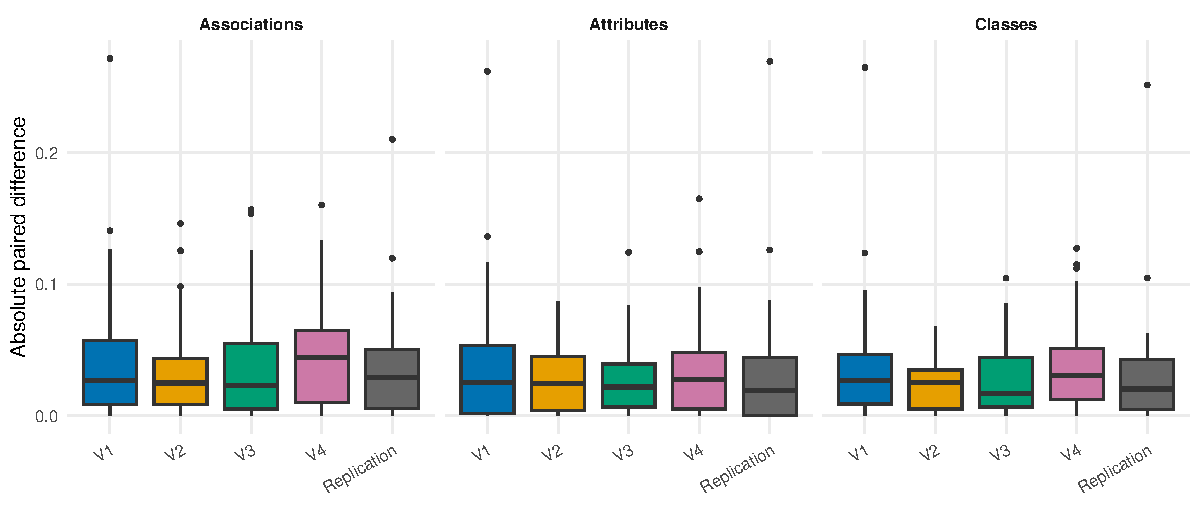
\includegraphics[width=\linewidth,height=0.30\textheight,keepaspectratio]{figures/fig6_absolute_differences.pdf}\par\small Absolute condition-associated and replication differences; boxes show medians and interquartile ranges.\end{center}
A conservative normal-approximation sensitivity calculation used two-sided alpha 0.05/12, 80\% power, and the observed standard deviation of paired differences. Approximate minimum detectable mean effects ranged from 0.019 to 0.037 score units. These are conditional planning approximations, not exact Wilcoxon power calculations or evidence for the null hypothesis. Detailed per-contrast values and all-available-pair and sign-test sensitivity results are exported separately.
\newpage
\subsection{Case-level heterogeneity and limitations}
V1/Associations: 25 improved, 4 exactly unchanged, 15 worsened; V1/Attributes: 20 improved, 8 exactly unchanged, 16 worsened; V1/Classes: 22 improved, 2 exactly unchanged, 20 worsened; V2/Associations: 27 improved, 7 exactly unchanged, 10 worsened; V2/Attributes: 17 improved, 8 exactly unchanged, 19 worsened; V2/Classes: 19 improved, 5 exactly unchanged, 20 worsened; V3/Associations: 20 improved, 4 exactly unchanged, 20 worsened; V3/Attributes: 15 improved, 7 exactly unchanged, 22 worsened; V3/Classes: 19 improved, 1 exactly unchanged, 24 worsened; V4/Associations: 17 improved, 3 exactly unchanged, 24 worsened; V4/Attributes: 15 improved, 1 exactly unchanged, 28 worsened; V4/Classes: 14 improved, 1 exactly unchanged, 29 worsened
. Opposing case-level changes can cancel in the aggregate; an unchanged score does not establish an identical diagram.
The optional random-intercept analysis was not run because lmerTest was unavailable. No variance-component claim is made.
\begin{center}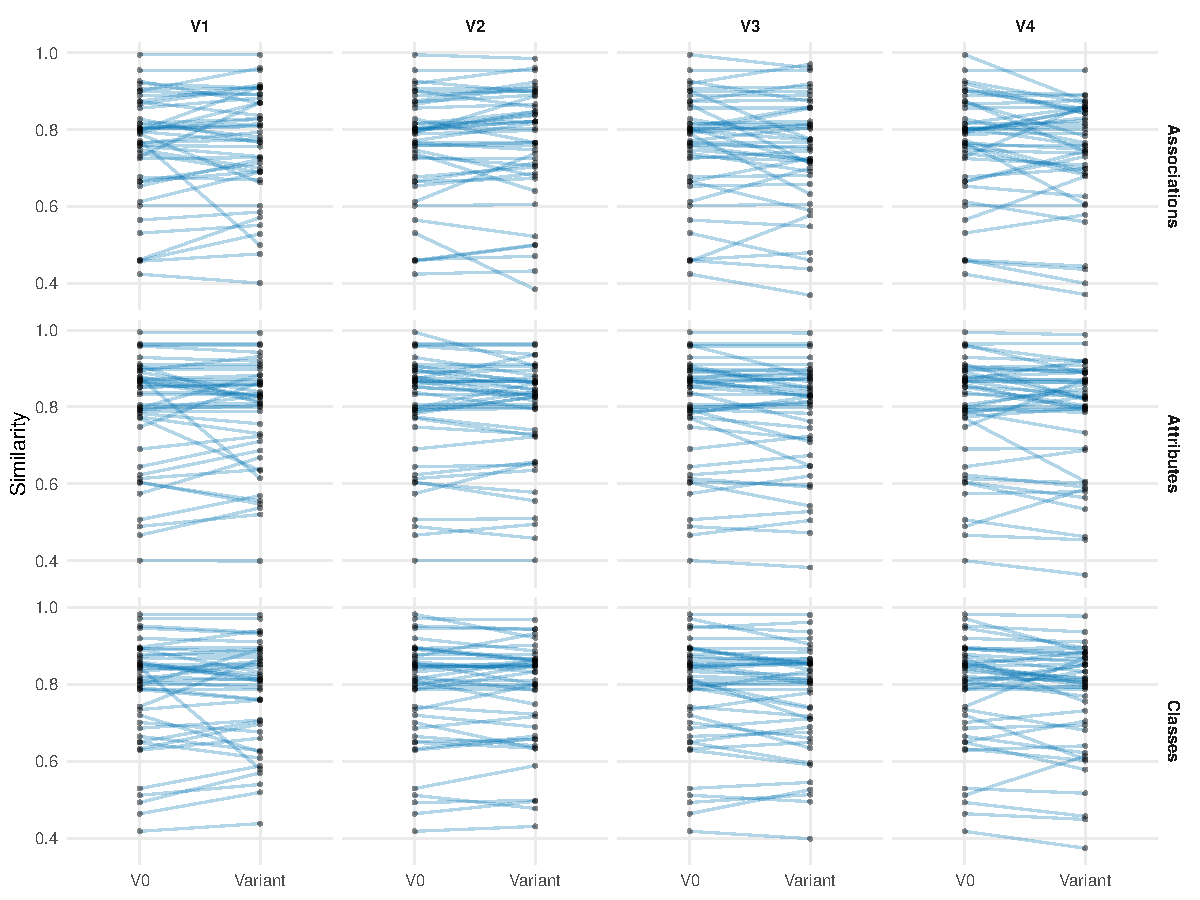
\includegraphics[width=\linewidth,height=0.36\textheight,keepaspectratio]{figures/fig2_paired_case_changes.pdf}\par\small Within-case baseline-to-variant changes, separated by metric and condition.\end{center}
Only one generation was obtained per manipulated condition and case. Individual changes cannot be separated cleanly into condition effects and stochastic generation variability. The second V0 run does not estimate condition-specific repeat variance. No independent manipulation check is present in the supplied files. Complete-case inference conditions on evaluability, and benchmark cases are not a random sample of all possible domain descriptions. Non-significance does not demonstrate equivalence or an ability to resolve every ambiguity. The metric measures reference similarity, not every aspect of semantic correctness.
